\chapter{Algebra}
A refresher on relevant basic algebra and number theory. Maybe some can be used in the thesis or as an appendix.

\section{Rings}
A polynomial with coefficients in $\mathbb{F}$ is denoted $\mathbb{F}[X]$. The quotient of a ring $\mathbb{F}[X]/{S}$ is just $\mathbb{F}[X] \bmod{S}$. Most FHE schemes are based on rings (\gls{rlwe}, \gls{rgsw} etc.), and in particular we often see the ring $(\mathbb{Z}/q\mathbb{Z})[X] / (f(X))$ for some integer $q$ and some polynomial $f(X)$. Here $(\mathbb{Z}/q\mathbb{Z})[X]$ denotes a polynomial with coefficients in $\mathbb{Z}_q$ i.e. integers mod $q$, and since we have $\mathbb{Z}_q[X]/(f(X))$ it means that $f(x) \equiv 0$ in this ring. A natural choice is $f(X) = X^n + 1$ for many of these schemes for some variable $n$, as this allows all polynomials with degree (up to) $n$. (And is a cyclotomic polynomial $\to$ has additional structure that can be used to optimize performance.)

If $f(X)$ is irreducible over $\mathbb{F}$, then $\mathbb{F}[X]/(f(X))$ is a field. (And $f(X)$ is a maximum ideal of $\mathbb{F}[X]$.)

\textcolor{red}{A factor group $G/H$, pronounced \emph{G mod H}, is a factor group where $H$ \textbf{is the identity element}.} In other words, $\mathbb{F}[X]/(f(X))$ has the (additive) identity $f(X)$ aka. $f(X) \equiv 0$ in the ring.

\section{Cyclotomic Polynomials}
$(X^n + 1)$ is a \emph{cyclotomic polynomial}.
They are irreducible over $\mathbb{Z}$ as long as $n = 2^m,\; m\in\mathbb{Z}$ (in other words, $n$ is a power of 2) but are typically not irreducible over $\mathbb{Z}_q$.

\begin{definition}
    \label{def:roots-of-unity}
    For any positive integer $n$, the $n$-th roots of unity are the (complex) solutions to the equation $x^n = 1$, and there are $n$ solutions to the equation.
\end{definition}

Let $\zeta_n(x) = e^{2\pi i}$. It follows from Euler's formula $e^{2\pi i} = \sin{2\pi} + i\cos{2\pi} = 1$ that $\zeta_n^k(x) = \{1, e^{2\pi i}, e^{4\pi i}, \dots, e^{2k\pi i}\}$ for $0 \leq k < n$ are the $n$-th roots of unity. At least this is the case over $\mathbb{C}$, but we can define the same problem over different fields.

Geometrically, we can interpret the $n$-th roots of unity as the points that are evenly spread on the unit circle in the complex plane, starting from 1 on the real axis. (The word \emph{cyclotomic} means \emph{circle-dividing}.) 

\begin{figure}[ht!]
    \centering
    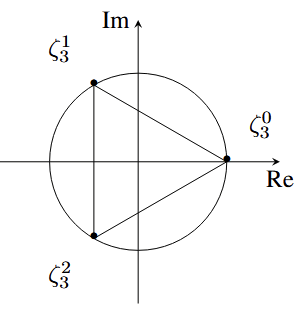
\includegraphics[width=0.33\linewidth]{figs/cyclotomic-temp.png}
    \caption{TODO: Create in tikz or drop}
    \label{fig:cyclotomic:1}
\end{figure}

We can define this notion of different fields, and are most interested in defining it over a \emph{finite} $\mathbb{Z}_{p^k}$. As an example, consider $\mathbb{Z}_7 = \{0,1,2,3,4,5,6\}$. The 4-th roots of unity are only 1 and 6, as these are the only values equivalent to 1 when raised to the fourth power. Note that this field has $\phi(n)=\phi(4)=2$ number of $n$-th roots for $n=4$. This is always the case for any finite field and choice of $n$. 

\begin{align}
    1^4 &\equiv 1 \mod{7} \\
    6^4 &\equiv 1 \mod{7}
\end{align}

\begin{theorem}
    A finite field $\mathbb{Z}_{p^k}$ has a primitive $n$-th root if and only if $n\,|\,(p^k -1)$. In this case, there are $\phi(n)$ roots of unity! 
\end{theorem}

\begin{definition}
    An $n$-th root of unity $r$ is called \emph{primitive} if it is not a $d$-th root of unity for any integer $d$ smaller than $n$.
\end{definition}

\begin{theorem}
    The $n$-th primitive roots of unity are precisely:
    \begin{equation}
    \label{eq:primitive-roots}
        \{\zeta_n^k\,:\,1\leq k \leq n - 1,\;\gcd(k,n) = 1\}    
    \end{equation}
\end{theorem}

\begin{definition}
    The $n$-th cyclotomic polynomial $\Phi_n(x)$ has the $n$-th primitive roots of unity as its roots: 
    \begin{equation}
        \Phi_n(x) = \prod_{\underset{\gcd(k,n)=1}{1 \leq k < n}} (x - \zeta_n^k)
    \end{equation}
\end{definition}

Again, we care only about a special class of cyclotomic polynomials that simplify our work. One step in this direction is considering only when $n$ is prime:

\begin{equation}
    \label{eq:cyclotomic:p}
    \Phi_n(x) = x^{n-1} + x^{n-2} + \dots + 1 = \sum_{t=0}^{n-1}x^t
\end{equation}

Now we consider only finite fields $\mathbb{GF}(p^k)$. Then the cyclotomic polynomials look like:

\begin{equation}
    \label{eq:cyclotomic:pk}
    \Phi_n(x) = \Phi_p(x^{n/p}) = \Phi_p(x^{p^{k-1}}) = \sum_{t=0}^{p-1}x^{tp^{k-1}}
\end{equation}

And finally, when $p=2$ so $n=2^k$ we get \eqref{eq:cyclotomic:2k} where $m=2^{k-1},\,n=2m,$.

\begin{equation}
    \label{eq:cyclotomic:2k}   
    \Phi_n(x) = x^m+1
\end{equation}

Cyclotomic polynomials are monic (implied by the definition) and has $\phi(n)$ linear factors. In addition, $\Phi_n(x)$ divides $x^n-1$. This implies an important relationship:

\begin{equation}
    \label{eq:cyclotomic:ident}
    x^n-1 = \prod_{d|n} \Phi_d(x)    
\end{equation}

The identity \eqref{eq:cyclotomic:ident} says that a number is an $n$-th root of unity iff. it is a $d$-th primitive root of unity for some natural number $d$ that divides $n$.



\section{Galois Group of Cyclotomic Polynomials}
Galois theory can be used to answer the question of whether the roots of an arbitrary polynomial $f$ can be expressed in terms of its coefficients. The method for doing so leads to the definition of the \emph{splitting field of a polynomial}, which contains the elementary symmetric polynomials and other polynomials of (subsets of) the roots that can be obtained from them??

\begin{definition}
    Let $f$ be a polynomial with rational coefficents. The splitting field $K$ of $f$ is the smallest field that contains the roots of $f$.
\end{definition}

$K$ is called the splitting field of $f$ because we can split $f$ into linear factors in $K$.

